\documentclass{article}
\setlength{\parindent}{0pt}
\setlength{\parskip}{2ex plus 0.5ex minus 0.2ex}
\usepackage[margin=1in]{geometry}
\renewcommand{\topfraction}{0.9}
\renewcommand{\bottomfraction}{0.8}
\setcounter{topnumber}{2}
\setcounter{bottomnumber}{2}
\setcounter{totalnumber}{4}
\renewcommand{\textfraction}{0.07}
\renewcommand{\floatpagefraction}{0.7}
\usepackage{graphicx}
\usepackage{textcomp}
\usepackage{placeins}
\usepackage[T1]{fontenc}
\usepackage{gensymb}
\usepackage[utf8]{inputenc}
\usepackage{caption}
\usepackage[export]{adjustbox}
\graphicspath{{./figures/}}
% hyperref usually has to go last
\usepackage[hidelinks]{hyperref}
% but glossaries behaves best if after hyperref
\usepackage[acronym,toc]{glossaries}
\include{acros}
\makeglossaries
% cleveref only behaves if after hyperref & glossaries
\usepackage{cleveref}

\let\Oldsection\section
\renewcommand{\section}{\FloatBarrier\Oldsection}

\let\Oldsubsection\subsection
\renewcommand{\subsection}{\FloatBarrier\Oldsubsection}

\let\Oldsubsubsection\subsubsection
\renewcommand{\subsubsection}{\FloatBarrier\Oldsubsubsection}

\newcommand{\code}[1]{\texttt{#1}}

\title{Introduction to Moltres: an Application for Simulation of Molten Salt Reactors}
\author{Alexander Lindsay, Kathryn Huff}

\begin{document}
\maketitle

\section{Model Description}

As a proof of concept and to ease resolution of strong transient gradients in
temperature between fuel and moderator, the physical three dimensional problem
is reduced to a two dimensional axisymmetric model. The model molten salt
reactor is based on the \gls{MSRE}. To approximately simulate the lattice
structure of the \gls{MSRE}, a geometry is constructed with 14 repeating
fuel-moderator regions, as shown in \cref{fig:geom}. The fuel and moderator
radii are chosen such that the resulting area/volume fraction of fuel is .225 as
for the \gls{MSRE}.

\begin{figure}
  \centering
  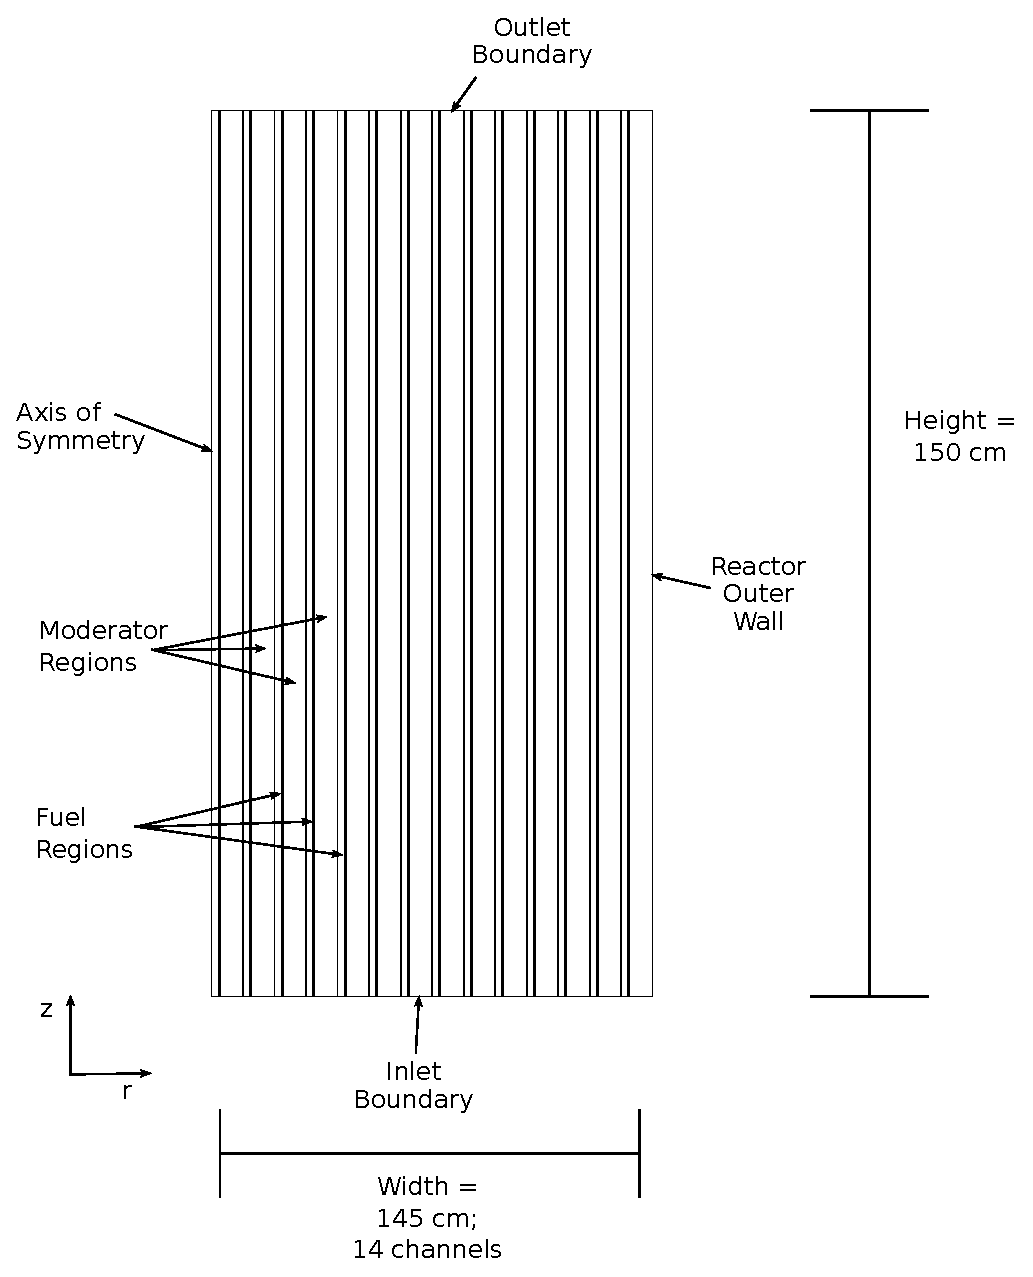
\includegraphics{geometry.eps}
  \label{fig:geom}
  \caption{A sketch of the \gls{MSR} model geometry}
\end{figure}

The model is implemented using the MOOSE \cite{gaston_physics-based_2015} application code
Moltres. \cite{lindsayad_arfc/moltres_nodate} Building on the massively
parallelizable MOOSE framework allows Moltres to be run on super-computing
platforms like \gls{NCSA}'s Blue Waters. For some three-dimensional simulations
(results not discussed here), the number of elements in the mesh and total
number of degrees of freedom exceed one million and ten million respectively. To
handle problems of this size, Moltres has been run on up to 608 cores. However,
reducing the problem dimension from three to two and using a structured mesh
that can be much more coarse in the axial direction allows problem solution to
be carried out on a single core in under five minutes.

The Moltres code-base currently includes kernels and boundary conditions for
solving for neutron fluxes, temperature, and precursor concentrations. In MOOSE
jargon, kernels are C++ classes that contain methods for computing residual and
Jacobian contributions corresponding to individual piecies of governing
equations. Developing the code-base in this way allows very modular construction
of equation systems; e.g. the same kernel that is used to represent heat
conduction can also be used to represent generic chemical diffusion. Moltres
also features neutron and precursor ``actions.'' These actions enable automatic
construction of the systems of equations for an arbitrary number of neutron and
precursor groups. This means that as long as group constants are provided in an appropriate
tabular form, a user only has to modify a couple of lines in a Moltres input
file to change from say two to fourty-four neutron groups.

In Moltres, neutrons are described with time-dependent multi-group diffusion theory as shown
in \cref{eq:neutrons}:

\begin{equation}
%% \frac{1}{v_g}\frac{\partial \phi_g}{\partial t} - \nabla \cdot D_g \nabla \phi_g
%% + \Sigma_g^r \phi_g = \sum_{g \ne g'}^G \Sigma_{g'\rightarrow g}^s \phi_{g'} + \chi_g^p \sum_{g' = 1}^G (1 - \beta)
%% \nu \Sigma_{g'}^f \phi_{g'}
\frac{1}{v_g}\frac{\partial \phi_g}{\partial t} - \nabla \cdot D_g \nabla \phi_g
+ \Sigma_g^r \phi_g = \sum_{g \ne g'}^G \Sigma_{g'\rightarrow g}^s \phi_{g'} + \chi_g^p \sum_{g' = 1}^G (1 - \beta)
\nu \Sigma_{g'}^f \phi_{g'} + \chi_g^d \sum_i^I \lambda_i C_i
\label{eq:neutrons}
\end{equation}

Delayed neutron precursors are described by \cref{eq:precursors}:

\begin{equation}
\frac{\partial C_i}{\partial t} = \sum_{g'= 1}^G \beta_i \nu \Sigma_{g'}^f
\phi_{g'} - \lambda_i C_i - \frac{\partial}{\partial z} u C_i
\label{eq:precursors}
\end{equation}

with the last term representing the effect of fuel advection. The governing
equation for the temperature is given by:

\begin{equation}
  \rho_fc_{p,f}\frac{\partial T_f}{\partial t} + \nabla\cdot\left(\rho_f c_{p,f}
  \vec{u}\cdot T_f -k_f\nabla T_f\right) =  Q_f
  \label{eq:fuel_temp}
\end{equation}

in the fuel and by:

\begin{equation}
  \rho_gc_{p,g}\frac{\partial T_g}{\partial t} + \nabla\cdot\left(-k_g\nabla T_g\right) =  Q_g
  \label{eq:moderator_temp}
\end{equation}

in the moderator. $Q_f$ is defined by:

\begin{equation}
  Q_f = \sum_{g=1}^G \epsilon_{f,g}\Sigma_{f,g}\phi_g
  \label{eq:fuel_source}
\end{equation}

and $Q_g$ is equal to $\gamma Q_f$, representing heat dissipation by gamma and
neutron irradiation in the moderator.

Reactor composition is based on the enriched uranium design for the \gls{MSRE}
and is given in \cref{table:comp}. \cite{robertson_msre_1965} Group constants
are generated with either Serpent \cite{leppanen_serpent_2015} or Scale
\cite{dehart_reactor_2011}. Temperature vs group constant interpolation tables
are constructed separately for fuel and moderator regions.

\begin{table}[htpb]
  \begin{center}
    \begin{tabular}{l | r}
      Component & Mass Fraction\\\hline\hline
      Li-7 & .1090\\
      Li-6 & 5$\cdot$10$^{-6}$\\
      F-19 & .6680\\
      Be-9 & .0627\\
      U-235 & .0167\\
      U-238 & .0344\\
    \end{tabular}
  \end{center}
  \caption{Fuel salt composition based on enriched Uranium \gls{MSRE} design \cite{robertson_msre_1965}
  \label{table:comp}
\end{table}


\section{Results \& Discussion}

Group fluxes are shown in \cref{fig:group1,fig:group2}. The effect of the vacuum
boundary conditions is shown clearly in the cosinusoidal shapes in radial and
axial directions. Striations are observed in both fast and thermal fluxes, with
the fast group preferring the fuel and the thermal group preferring the moderator.

\begin{figure}
  \centering
  \includegraphics{auto_diff_rho_group1.eps}
  \caption{Group 1 flux}
  \label{fig:group1}
\end{figure}

\begin{figure}
  \centering
  \includegraphics{auto_diff_rho_group2.eps}
  \caption{Group 2 flux}
  \label{fig:group2}
\end{figure}

The effect of the advecting fuel is seen in {fig:temp} where the temperature
rises steadily with increasing z-coordinate. As one might expect, the temperature
gradient is negative in the radial direction.

\begin{figure}
  \centering
  \includegraphics{auto_diff_rho_temp.eps}
  \caption{Temperature}
  \label{fig:temp}
\end{figure}

\Cref{fig:pre1} shows the concentration of the longest lived precursor in the
reactor. Not surprisingly, the channel concentrations are higher in fuel channels
with higher neutron fluxes and consequently a higher number of fission
events. Because of the small decay constant of the precursor, the maximum
concentration in any given channel occurs at the core outlet.

% Fix me! Precursor concentrations have goofy scaling
\begin{figure}
  \centering
  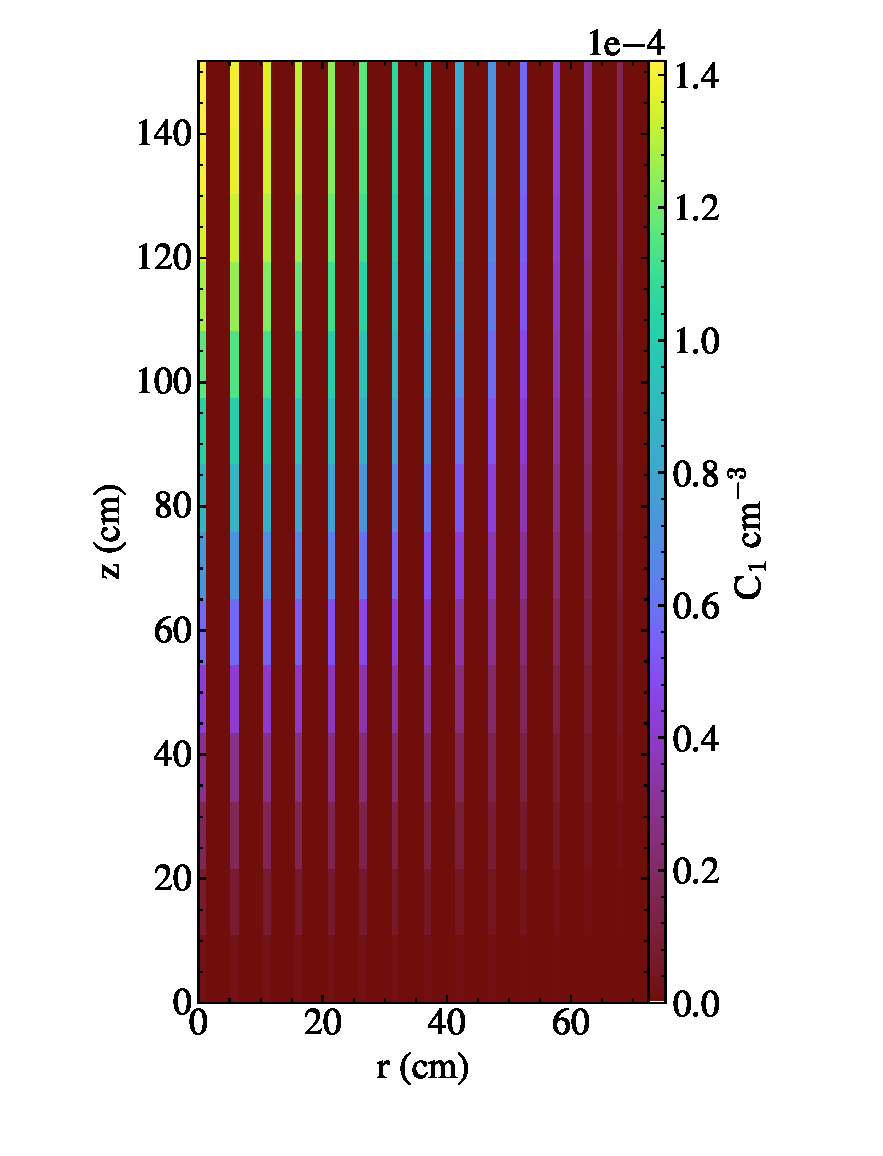
\includegraphics{auto_diff_rho_pre1.eps}
  \caption{Longest lived precursor concentration}
  \label{fig:pre1}
\end{figure}

With its much larger decay constant, the sixth and last precursor has its
maximum concentration around the center-plane of the reactor as shown in
\cref{fig:pre6}. As for all other precursors, its concentration decreases with
increasing radius and decreasing neutron flux.

% Fix me! Precursor concentrations have goofy scaling
\begin{figure}
  \centering
  \includegraphics{auto_diff_rho_pre6.eps}
  \caption{Shortest lived precursor concentration}
  \label{fig:pre6}
\end{figure}

\FloatBarrier
\clearpage
\printglossary[type=\acronymtype]
\bibliographystyle{unsrt}
\bibliography{Moltres}
\end{document}
